

\tikzset{every picture/.style={line width=0.75pt}} %set default line width to 0.75pt        

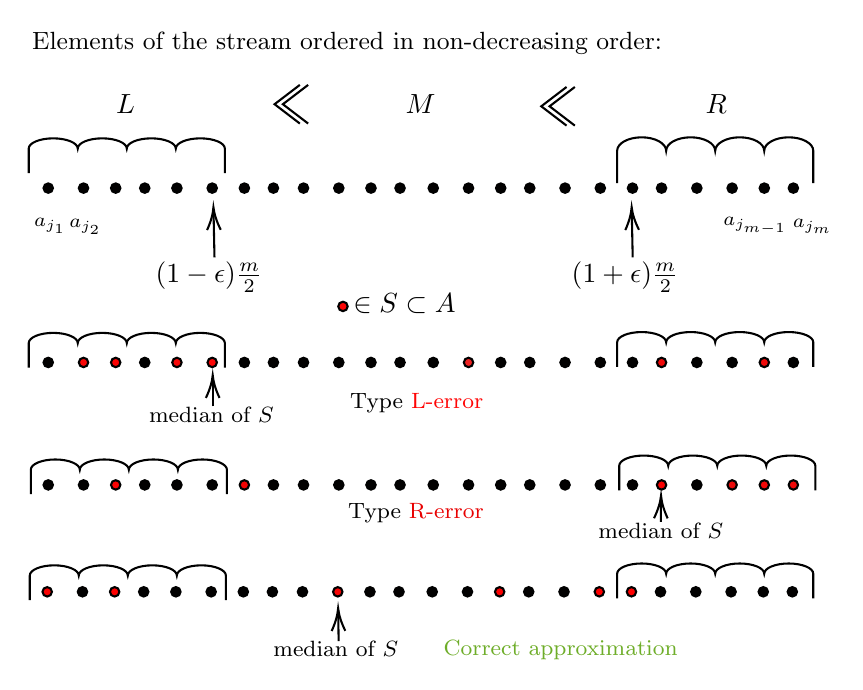
\begin{tikzpicture}[x=0.75pt,y=0.75pt,yscale=-1,xscale=1]
%uncomment if require: \path (0,442); %set diagram left start at 0, and has height of 442

%Shape: Circle [id:dp8581968473092385] 
\draw  [fill={rgb, 255:red, 2; green, 1; blue, 1 }  ,fill opacity=1 ] (98,150.22) .. controls (98,148.97) and (99.02,147.95) .. (100.28,147.95) .. controls (101.53,147.95) and (102.55,148.97) .. (102.55,150.22) .. controls (102.55,151.48) and (101.53,152.5) .. (100.28,152.5) .. controls (99.02,152.5) and (98,151.48) .. (98,150.22) -- cycle ;
%Shape: Circle [id:dp6208581543375671] 
\draw  [fill={rgb, 255:red, 2; green, 1; blue, 1 }  ,fill opacity=1 ] (130.5,150.22) .. controls (130.5,148.97) and (131.52,147.95) .. (132.78,147.95) .. controls (134.03,147.95) and (135.05,148.97) .. (135.05,150.22) .. controls (135.05,151.48) and (134.03,152.5) .. (132.78,152.5) .. controls (131.52,152.5) and (130.5,151.48) .. (130.5,150.22) -- cycle ;
%Shape: Circle [id:dp4607760483214204] 
\draw  [fill={rgb, 255:red, 2; green, 1; blue, 1 }  ,fill opacity=1 ] (115,150.22) .. controls (115,148.97) and (116.02,147.95) .. (117.28,147.95) .. controls (118.53,147.95) and (119.55,148.97) .. (119.55,150.22) .. controls (119.55,151.48) and (118.53,152.5) .. (117.28,152.5) .. controls (116.02,152.5) and (115,151.48) .. (115,150.22) -- cycle ;
%Shape: Circle [id:dp27752749632415497] 
\draw  [fill={rgb, 255:red, 2; green, 1; blue, 1 }  ,fill opacity=1 ] (144.5,150.22) .. controls (144.5,148.97) and (145.52,147.95) .. (146.78,147.95) .. controls (148.03,147.95) and (149.05,148.97) .. (149.05,150.22) .. controls (149.05,151.48) and (148.03,152.5) .. (146.78,152.5) .. controls (145.52,152.5) and (144.5,151.48) .. (144.5,150.22) -- cycle ;
%Shape: Circle [id:dp7060609257826158] 
\draw  [fill={rgb, 255:red, 2; green, 1; blue, 1 }  ,fill opacity=1 ] (160,150.22) .. controls (160,148.97) and (161.02,147.95) .. (162.28,147.95) .. controls (163.53,147.95) and (164.55,148.97) .. (164.55,150.22) .. controls (164.55,151.48) and (163.53,152.5) .. (162.28,152.5) .. controls (161.02,152.5) and (160,151.48) .. (160,150.22) -- cycle ;
%Shape: Circle [id:dp8024176947646371] 
\draw  [fill={rgb, 255:red, 2; green, 1; blue, 1 }  ,fill opacity=1 ] (192.5,150.22) .. controls (192.5,148.97) and (193.52,147.95) .. (194.78,147.95) .. controls (196.03,147.95) and (197.05,148.97) .. (197.05,150.22) .. controls (197.05,151.48) and (196.03,152.5) .. (194.78,152.5) .. controls (193.52,152.5) and (192.5,151.48) .. (192.5,150.22) -- cycle ;
%Shape: Circle [id:dp843376660730378] 
\draw  [fill={rgb, 255:red, 2; green, 1; blue, 1 }  ,fill opacity=1 ] (177,150.22) .. controls (177,148.97) and (178.02,147.95) .. (179.28,147.95) .. controls (180.53,147.95) and (181.55,148.97) .. (181.55,150.22) .. controls (181.55,151.48) and (180.53,152.5) .. (179.28,152.5) .. controls (178.02,152.5) and (177,151.48) .. (177,150.22) -- cycle ;
%Shape: Circle [id:dp8995137192141623] 
\draw  [fill={rgb, 255:red, 2; green, 1; blue, 1 }  ,fill opacity=1 ] (206.5,150.22) .. controls (206.5,148.97) and (207.52,147.95) .. (208.78,147.95) .. controls (210.03,147.95) and (211.05,148.97) .. (211.05,150.22) .. controls (211.05,151.48) and (210.03,152.5) .. (208.78,152.5) .. controls (207.52,152.5) and (206.5,151.48) .. (206.5,150.22) -- cycle ;
%Shape: Circle [id:dp005871190997944198] 
\draw  [fill={rgb, 255:red, 2; green, 1; blue, 1 }  ,fill opacity=1 ] (221,150.22) .. controls (221,148.97) and (222.02,147.95) .. (223.28,147.95) .. controls (224.53,147.95) and (225.55,148.97) .. (225.55,150.22) .. controls (225.55,151.48) and (224.53,152.5) .. (223.28,152.5) .. controls (222.02,152.5) and (221,151.48) .. (221,150.22) -- cycle ;
%Shape: Circle [id:dp06985974018043584] 
\draw  [fill={rgb, 255:red, 2; green, 1; blue, 1 }  ,fill opacity=1 ] (253.5,150.22) .. controls (253.5,148.97) and (254.52,147.95) .. (255.78,147.95) .. controls (257.03,147.95) and (258.05,148.97) .. (258.05,150.22) .. controls (258.05,151.48) and (257.03,152.5) .. (255.78,152.5) .. controls (254.52,152.5) and (253.5,151.48) .. (253.5,150.22) -- cycle ;
%Shape: Circle [id:dp2791257096565082] 
\draw  [fill={rgb, 255:red, 2; green, 1; blue, 1 }  ,fill opacity=1 ] (238,150.22) .. controls (238,148.97) and (239.02,147.95) .. (240.28,147.95) .. controls (241.53,147.95) and (242.55,148.97) .. (242.55,150.22) .. controls (242.55,151.48) and (241.53,152.5) .. (240.28,152.5) .. controls (239.02,152.5) and (238,151.48) .. (238,150.22) -- cycle ;
%Shape: Circle [id:dp908479495856961] 
\draw  [fill={rgb, 255:red, 2; green, 1; blue, 1 }  ,fill opacity=1 ] (267.5,150.22) .. controls (267.5,148.97) and (268.52,147.95) .. (269.78,147.95) .. controls (271.03,147.95) and (272.05,148.97) .. (272.05,150.22) .. controls (272.05,151.48) and (271.03,152.5) .. (269.78,152.5) .. controls (268.52,152.5) and (267.5,151.48) .. (267.5,150.22) -- cycle ;
%Shape: Circle [id:dp09490854627786505] 
\draw  [fill={rgb, 255:red, 2; green, 1; blue, 1 }  ,fill opacity=1 ] (283.5,150.22) .. controls (283.5,148.97) and (284.52,147.95) .. (285.78,147.95) .. controls (287.03,147.95) and (288.05,148.97) .. (288.05,150.22) .. controls (288.05,151.48) and (287.03,152.5) .. (285.78,152.5) .. controls (284.52,152.5) and (283.5,151.48) .. (283.5,150.22) -- cycle ;
%Shape: Circle [id:dp5505733462825663] 
\draw  [fill={rgb, 255:red, 2; green, 1; blue, 1 }  ,fill opacity=1 ] (316,150.22) .. controls (316,148.97) and (317.02,147.95) .. (318.28,147.95) .. controls (319.53,147.95) and (320.55,148.97) .. (320.55,150.22) .. controls (320.55,151.48) and (319.53,152.5) .. (318.28,152.5) .. controls (317.02,152.5) and (316,151.48) .. (316,150.22) -- cycle ;
%Shape: Circle [id:dp4528785997557584] 
\draw  [fill={rgb, 255:red, 2; green, 1; blue, 1 }  ,fill opacity=1 ] (300.5,150.22) .. controls (300.5,148.97) and (301.52,147.95) .. (302.78,147.95) .. controls (304.03,147.95) and (305.05,148.97) .. (305.05,150.22) .. controls (305.05,151.48) and (304.03,152.5) .. (302.78,152.5) .. controls (301.52,152.5) and (300.5,151.48) .. (300.5,150.22) -- cycle ;
%Shape: Circle [id:dp2678446713324063] 
\draw  [fill={rgb, 255:red, 2; green, 1; blue, 1 }  ,fill opacity=1 ] (330,150.22) .. controls (330,148.97) and (331.02,147.95) .. (332.28,147.95) .. controls (333.53,147.95) and (334.55,148.97) .. (334.55,150.22) .. controls (334.55,151.48) and (333.53,152.5) .. (332.28,152.5) .. controls (331.02,152.5) and (330,151.48) .. (330,150.22) -- cycle ;
%Shape: Circle [id:dp5073441056046755] 
\draw  [fill={rgb, 255:red, 2; green, 1; blue, 1 }  ,fill opacity=1 ] (347,150.22) .. controls (347,148.97) and (348.02,147.95) .. (349.28,147.95) .. controls (350.53,147.95) and (351.55,148.97) .. (351.55,150.22) .. controls (351.55,151.48) and (350.53,152.5) .. (349.28,152.5) .. controls (348.02,152.5) and (347,151.48) .. (347,150.22) -- cycle ;
%Shape: Circle [id:dp2845339833010009] 
\draw  [fill={rgb, 255:red, 2; green, 1; blue, 1 }  ,fill opacity=1 ] (379.5,150.22) .. controls (379.5,148.97) and (380.52,147.95) .. (381.78,147.95) .. controls (383.03,147.95) and (384.05,148.97) .. (384.05,150.22) .. controls (384.05,151.48) and (383.03,152.5) .. (381.78,152.5) .. controls (380.52,152.5) and (379.5,151.48) .. (379.5,150.22) -- cycle ;
%Shape: Circle [id:dp4535556857943255] 
\draw  [fill={rgb, 255:red, 2; green, 1; blue, 1 }  ,fill opacity=1 ] (364,150.22) .. controls (364,148.97) and (365.02,147.95) .. (366.28,147.95) .. controls (367.53,147.95) and (368.55,148.97) .. (368.55,150.22) .. controls (368.55,151.48) and (367.53,152.5) .. (366.28,152.5) .. controls (365.02,152.5) and (364,151.48) .. (364,150.22) -- cycle ;
%Shape: Circle [id:dp23357726940116785] 
\draw  [fill={rgb, 255:red, 2; green, 1; blue, 1 }  ,fill opacity=1 ] (393.5,150.22) .. controls (393.5,148.97) and (394.52,147.95) .. (395.78,147.95) .. controls (397.03,147.95) and (398.05,148.97) .. (398.05,150.22) .. controls (398.05,151.48) and (397.03,152.5) .. (395.78,152.5) .. controls (394.52,152.5) and (393.5,151.48) .. (393.5,150.22) -- cycle ;
%Shape: Circle [id:dp890755709027476] 
\draw  [fill={rgb, 255:red, 2; green, 1; blue, 1 }  ,fill opacity=1 ] (410.5,150.22) .. controls (410.5,148.97) and (411.52,147.95) .. (412.78,147.95) .. controls (414.03,147.95) and (415.05,148.97) .. (415.05,150.22) .. controls (415.05,151.48) and (414.03,152.5) .. (412.78,152.5) .. controls (411.52,152.5) and (410.5,151.48) .. (410.5,150.22) -- cycle ;
%Shape: Circle [id:dp813959068002973] 
\draw  [fill={rgb, 255:red, 2; green, 1; blue, 1 }  ,fill opacity=1 ] (443,150.22) .. controls (443,148.97) and (444.02,147.95) .. (445.28,147.95) .. controls (446.53,147.95) and (447.55,148.97) .. (447.55,150.22) .. controls (447.55,151.48) and (446.53,152.5) .. (445.28,152.5) .. controls (444.02,152.5) and (443,151.48) .. (443,150.22) -- cycle ;
%Shape: Circle [id:dp5743495621854182] 
\draw  [fill={rgb, 255:red, 2; green, 1; blue, 1 }  ,fill opacity=1 ] (427.5,150.22) .. controls (427.5,148.97) and (428.52,147.95) .. (429.78,147.95) .. controls (431.03,147.95) and (432.05,148.97) .. (432.05,150.22) .. controls (432.05,151.48) and (431.03,152.5) .. (429.78,152.5) .. controls (428.52,152.5) and (427.5,151.48) .. (427.5,150.22) -- cycle ;
%Shape: Circle [id:dp5990552424970276] 
\draw  [fill={rgb, 255:red, 2; green, 1; blue, 1 }  ,fill opacity=1 ] (457,150.22) .. controls (457,148.97) and (458.02,147.95) .. (459.28,147.95) .. controls (460.53,147.95) and (461.55,148.97) .. (461.55,150.22) .. controls (461.55,151.48) and (460.53,152.5) .. (459.28,152.5) .. controls (458.02,152.5) and (457,151.48) .. (457,150.22) -- cycle ;
%Straight Lines [id:da19846509257508438] 
\draw    (180.37,183.57) -- (179.91,161.45) ;
\draw [shift={(179.87,159.45)}, rotate = 448.81] [color={rgb, 255:red, 0; green, 0; blue, 0 }  ][line width=0.75]    (10.93,-3.29) .. controls (6.95,-1.4) and (3.31,-0.3) .. (0,0) .. controls (3.31,0.3) and (6.95,1.4) .. (10.93,3.29)   ;
%Straight Lines [id:da9205396435469643] 
\draw    (381.87,183.57) -- (381.41,161.45) ;
\draw [shift={(381.37,159.45)}, rotate = 448.81] [color={rgb, 255:red, 0; green, 0; blue, 0 }  ][line width=0.75]    (10.93,-3.29) .. controls (6.95,-1.4) and (3.31,-0.3) .. (0,0) .. controls (3.31,0.3) and (6.95,1.4) .. (10.93,3.29)   ;
%Shape: Inductor [id:dp5152296175648501] 
\draw   (90.87,143) -- (90.87,131.18) .. controls (90.87,128.46) and (96.16,126.25) .. (102.68,126.25) .. controls (109.2,126.25) and (114.49,128.46) .. (114.49,131.18) .. controls (114.49,128.46) and (119.78,126.25) .. (126.3,126.25) .. controls (132.82,126.25) and (138.12,128.46) .. (138.12,131.18) .. controls (138.12,128.46) and (143.41,126.25) .. (149.93,126.25) .. controls (156.45,126.25) and (161.74,128.46) .. (161.74,131.18) .. controls (161.74,128.46) and (167.03,126.25) .. (173.55,126.25) .. controls (180.07,126.25) and (185.37,128.46) .. (185.37,131.18) -- (185.37,143) ;
%Shape: Inductor [id:dp8791138604675957] 
\draw   (374.37,147.84) -- (374.37,132.25) .. controls (374.37,128.66) and (379.66,125.75) .. (386.18,125.75) .. controls (392.7,125.75) and (397.99,128.66) .. (397.99,132.25) .. controls (397.99,128.66) and (403.28,125.75) .. (409.8,125.75) .. controls (416.32,125.75) and (421.62,128.66) .. (421.62,132.25) .. controls (421.62,128.66) and (426.91,125.75) .. (433.43,125.75) .. controls (439.95,125.75) and (445.24,128.66) .. (445.24,132.25) .. controls (445.24,128.66) and (450.53,125.75) .. (457.05,125.75) .. controls (463.57,125.75) and (468.87,128.66) .. (468.87,132.25) -- (468.87,147.84) ;
%Shape: Circle [id:dp7249199477515286] 
\draw  [fill={rgb, 255:red, 2; green, 1; blue, 1 }  ,fill opacity=1 ] (98,234.22) .. controls (98,232.97) and (99.02,231.95) .. (100.28,231.95) .. controls (101.53,231.95) and (102.55,232.97) .. (102.55,234.22) .. controls (102.55,235.48) and (101.53,236.5) .. (100.28,236.5) .. controls (99.02,236.5) and (98,235.48) .. (98,234.22) -- cycle ;
%Shape: Circle [id:dp411935093256652] 
\draw  [fill={rgb, 255:red, 252; green, 1; blue, 1 }  ,fill opacity=1 ] (130.5,234.22) .. controls (130.5,232.97) and (131.52,231.95) .. (132.78,231.95) .. controls (134.03,231.95) and (135.05,232.97) .. (135.05,234.22) .. controls (135.05,235.48) and (134.03,236.5) .. (132.78,236.5) .. controls (131.52,236.5) and (130.5,235.48) .. (130.5,234.22) -- cycle ;
%Shape: Circle [id:dp7698024479555919] 
\draw  [fill={rgb, 255:red, 249; green, 6; blue, 6 }  ,fill opacity=1 ] (115,234.22) .. controls (115,232.97) and (116.02,231.95) .. (117.28,231.95) .. controls (118.53,231.95) and (119.55,232.97) .. (119.55,234.22) .. controls (119.55,235.48) and (118.53,236.5) .. (117.28,236.5) .. controls (116.02,236.5) and (115,235.48) .. (115,234.22) -- cycle ;
%Shape: Circle [id:dp5565730609176603] 
\draw  [fill={rgb, 255:red, 0; green, 0; blue, 0 }  ,fill opacity=1 ] (144.5,234.22) .. controls (144.5,232.97) and (145.52,231.95) .. (146.78,231.95) .. controls (148.03,231.95) and (149.05,232.97) .. (149.05,234.22) .. controls (149.05,235.48) and (148.03,236.5) .. (146.78,236.5) .. controls (145.52,236.5) and (144.5,235.48) .. (144.5,234.22) -- cycle ;
%Shape: Circle [id:dp5445256521850119] 
\draw  [fill={rgb, 255:red, 247; green, 8; blue, 8 }  ,fill opacity=1 ] (160,234.22) .. controls (160,232.97) and (161.02,231.95) .. (162.28,231.95) .. controls (163.53,231.95) and (164.55,232.97) .. (164.55,234.22) .. controls (164.55,235.48) and (163.53,236.5) .. (162.28,236.5) .. controls (161.02,236.5) and (160,235.48) .. (160,234.22) -- cycle ;
%Shape: Circle [id:dp9891697464651006] 
\draw  [fill={rgb, 255:red, 2; green, 1; blue, 1 }  ,fill opacity=1 ] (192.5,234.22) .. controls (192.5,232.97) and (193.52,231.95) .. (194.78,231.95) .. controls (196.03,231.95) and (197.05,232.97) .. (197.05,234.22) .. controls (197.05,235.48) and (196.03,236.5) .. (194.78,236.5) .. controls (193.52,236.5) and (192.5,235.48) .. (192.5,234.22) -- cycle ;
%Shape: Circle [id:dp7019842655108118] 
\draw  [fill={rgb, 255:red, 252; green, 6; blue, 6 }  ,fill opacity=1 ] (177,234.22) .. controls (177,232.97) and (178.02,231.95) .. (179.28,231.95) .. controls (180.53,231.95) and (181.55,232.97) .. (181.55,234.22) .. controls (181.55,235.48) and (180.53,236.5) .. (179.28,236.5) .. controls (178.02,236.5) and (177,235.48) .. (177,234.22) -- cycle ;
%Shape: Circle [id:dp4597877230884737] 
\draw  [fill={rgb, 255:red, 2; green, 1; blue, 1 }  ,fill opacity=1 ] (206.5,234.22) .. controls (206.5,232.97) and (207.52,231.95) .. (208.78,231.95) .. controls (210.03,231.95) and (211.05,232.97) .. (211.05,234.22) .. controls (211.05,235.48) and (210.03,236.5) .. (208.78,236.5) .. controls (207.52,236.5) and (206.5,235.48) .. (206.5,234.22) -- cycle ;
%Shape: Circle [id:dp08704872547158637] 
\draw  [fill={rgb, 255:red, 2; green, 1; blue, 1 }  ,fill opacity=1 ] (221,234.22) .. controls (221,232.97) and (222.02,231.95) .. (223.28,231.95) .. controls (224.53,231.95) and (225.55,232.97) .. (225.55,234.22) .. controls (225.55,235.48) and (224.53,236.5) .. (223.28,236.5) .. controls (222.02,236.5) and (221,235.48) .. (221,234.22) -- cycle ;
%Shape: Circle [id:dp9295783908060651] 
\draw  [fill={rgb, 255:red, 2; green, 1; blue, 1 }  ,fill opacity=1 ] (253.5,234.22) .. controls (253.5,232.97) and (254.52,231.95) .. (255.78,231.95) .. controls (257.03,231.95) and (258.05,232.97) .. (258.05,234.22) .. controls (258.05,235.48) and (257.03,236.5) .. (255.78,236.5) .. controls (254.52,236.5) and (253.5,235.48) .. (253.5,234.22) -- cycle ;
%Shape: Circle [id:dp45928791636051214] 
\draw  [fill={rgb, 255:red, 2; green, 1; blue, 1 }  ,fill opacity=1 ] (238,234.22) .. controls (238,232.97) and (239.02,231.95) .. (240.28,231.95) .. controls (241.53,231.95) and (242.55,232.97) .. (242.55,234.22) .. controls (242.55,235.48) and (241.53,236.5) .. (240.28,236.5) .. controls (239.02,236.5) and (238,235.48) .. (238,234.22) -- cycle ;
%Shape: Circle [id:dp05626705918080788] 
\draw  [fill={rgb, 255:red, 2; green, 1; blue, 1 }  ,fill opacity=1 ] (267.5,234.22) .. controls (267.5,232.97) and (268.52,231.95) .. (269.78,231.95) .. controls (271.03,231.95) and (272.05,232.97) .. (272.05,234.22) .. controls (272.05,235.48) and (271.03,236.5) .. (269.78,236.5) .. controls (268.52,236.5) and (267.5,235.48) .. (267.5,234.22) -- cycle ;
%Shape: Circle [id:dp15688207983640168] 
\draw  [fill={rgb, 255:red, 2; green, 1; blue, 1 }  ,fill opacity=1 ] (283.5,234.22) .. controls (283.5,232.97) and (284.52,231.95) .. (285.78,231.95) .. controls (287.03,231.95) and (288.05,232.97) .. (288.05,234.22) .. controls (288.05,235.48) and (287.03,236.5) .. (285.78,236.5) .. controls (284.52,236.5) and (283.5,235.48) .. (283.5,234.22) -- cycle ;
%Shape: Circle [id:dp36962261876256497] 
\draw  [fill={rgb, 255:red, 2; green, 1; blue, 1 }  ,fill opacity=1 ] (316,234.22) .. controls (316,232.97) and (317.02,231.95) .. (318.28,231.95) .. controls (319.53,231.95) and (320.55,232.97) .. (320.55,234.22) .. controls (320.55,235.48) and (319.53,236.5) .. (318.28,236.5) .. controls (317.02,236.5) and (316,235.48) .. (316,234.22) -- cycle ;
%Shape: Circle [id:dp5050698879850942] 
\draw  [fill={rgb, 255:red, 237; green, 34; blue, 34 }  ,fill opacity=1 ] (300.5,234.22) .. controls (300.5,232.97) and (301.52,231.95) .. (302.78,231.95) .. controls (304.03,231.95) and (305.05,232.97) .. (305.05,234.22) .. controls (305.05,235.48) and (304.03,236.5) .. (302.78,236.5) .. controls (301.52,236.5) and (300.5,235.48) .. (300.5,234.22) -- cycle ;
%Shape: Circle [id:dp6680484042862456] 
\draw  [fill={rgb, 255:red, 2; green, 1; blue, 1 }  ,fill opacity=1 ] (330,234.22) .. controls (330,232.97) and (331.02,231.95) .. (332.28,231.95) .. controls (333.53,231.95) and (334.55,232.97) .. (334.55,234.22) .. controls (334.55,235.48) and (333.53,236.5) .. (332.28,236.5) .. controls (331.02,236.5) and (330,235.48) .. (330,234.22) -- cycle ;
%Shape: Circle [id:dp47094571853189804] 
\draw  [fill={rgb, 255:red, 2; green, 1; blue, 1 }  ,fill opacity=1 ] (347,234.22) .. controls (347,232.97) and (348.02,231.95) .. (349.28,231.95) .. controls (350.53,231.95) and (351.55,232.97) .. (351.55,234.22) .. controls (351.55,235.48) and (350.53,236.5) .. (349.28,236.5) .. controls (348.02,236.5) and (347,235.48) .. (347,234.22) -- cycle ;
%Shape: Circle [id:dp04484140104668133] 
\draw  [fill={rgb, 255:red, 2; green, 1; blue, 1 }  ,fill opacity=1 ] (379.5,234.22) .. controls (379.5,232.97) and (380.52,231.95) .. (381.78,231.95) .. controls (383.03,231.95) and (384.05,232.97) .. (384.05,234.22) .. controls (384.05,235.48) and (383.03,236.5) .. (381.78,236.5) .. controls (380.52,236.5) and (379.5,235.48) .. (379.5,234.22) -- cycle ;
%Shape: Circle [id:dp856741171572465] 
\draw  [fill={rgb, 255:red, 2; green, 1; blue, 1 }  ,fill opacity=1 ] (364,234.22) .. controls (364,232.97) and (365.02,231.95) .. (366.28,231.95) .. controls (367.53,231.95) and (368.55,232.97) .. (368.55,234.22) .. controls (368.55,235.48) and (367.53,236.5) .. (366.28,236.5) .. controls (365.02,236.5) and (364,235.48) .. (364,234.22) -- cycle ;
%Shape: Circle [id:dp41347964171447815] 
\draw  [fill={rgb, 255:red, 239; green, 8; blue, 8 }  ,fill opacity=1 ] (393.5,234.22) .. controls (393.5,232.97) and (394.52,231.95) .. (395.78,231.95) .. controls (397.03,231.95) and (398.05,232.97) .. (398.05,234.22) .. controls (398.05,235.48) and (397.03,236.5) .. (395.78,236.5) .. controls (394.52,236.5) and (393.5,235.48) .. (393.5,234.22) -- cycle ;
%Shape: Circle [id:dp46216897498754794] 
\draw  [fill={rgb, 255:red, 2; green, 1; blue, 1 }  ,fill opacity=1 ] (410.5,234.22) .. controls (410.5,232.97) and (411.52,231.95) .. (412.78,231.95) .. controls (414.03,231.95) and (415.05,232.97) .. (415.05,234.22) .. controls (415.05,235.48) and (414.03,236.5) .. (412.78,236.5) .. controls (411.52,236.5) and (410.5,235.48) .. (410.5,234.22) -- cycle ;
%Shape: Circle [id:dp7116623374382753] 
\draw  [fill={rgb, 255:red, 239; green, 9; blue, 9 }  ,fill opacity=1 ] (443,234.22) .. controls (443,232.97) and (444.02,231.95) .. (445.28,231.95) .. controls (446.53,231.95) and (447.55,232.97) .. (447.55,234.22) .. controls (447.55,235.48) and (446.53,236.5) .. (445.28,236.5) .. controls (444.02,236.5) and (443,235.48) .. (443,234.22) -- cycle ;
%Shape: Circle [id:dp6499482610124566] 
\draw  [fill={rgb, 255:red, 2; green, 1; blue, 1 }  ,fill opacity=1 ] (427.5,234.22) .. controls (427.5,232.97) and (428.52,231.95) .. (429.78,231.95) .. controls (431.03,231.95) and (432.05,232.97) .. (432.05,234.22) .. controls (432.05,235.48) and (431.03,236.5) .. (429.78,236.5) .. controls (428.52,236.5) and (427.5,235.48) .. (427.5,234.22) -- cycle ;
%Shape: Circle [id:dp8145074031741266] 
\draw  [fill={rgb, 255:red, 2; green, 1; blue, 1 }  ,fill opacity=1 ] (457,234.22) .. controls (457,232.97) and (458.02,231.95) .. (459.28,231.95) .. controls (460.53,231.95) and (461.55,232.97) .. (461.55,234.22) .. controls (461.55,235.48) and (460.53,236.5) .. (459.28,236.5) .. controls (458.02,236.5) and (457,235.48) .. (457,234.22) -- cycle ;
%Shape: Circle [id:dp40046321332225754] 
\draw  [fill={rgb, 255:red, 2; green, 1; blue, 1 }  ,fill opacity=1 ] (98,293.22) .. controls (98,291.97) and (99.02,290.95) .. (100.28,290.95) .. controls (101.53,290.95) and (102.55,291.97) .. (102.55,293.22) .. controls (102.55,294.48) and (101.53,295.5) .. (100.28,295.5) .. controls (99.02,295.5) and (98,294.48) .. (98,293.22) -- cycle ;
%Shape: Circle [id:dp7217477715771097] 
\draw  [fill={rgb, 255:red, 251; green, 3; blue, 3 }  ,fill opacity=1 ] (130.5,293.22) .. controls (130.5,291.97) and (131.52,290.95) .. (132.78,290.95) .. controls (134.03,290.95) and (135.05,291.97) .. (135.05,293.22) .. controls (135.05,294.48) and (134.03,295.5) .. (132.78,295.5) .. controls (131.52,295.5) and (130.5,294.48) .. (130.5,293.22) -- cycle ;
%Shape: Circle [id:dp4044652681959163] 
\draw  [fill={rgb, 255:red, 2; green, 1; blue, 1 }  ,fill opacity=1 ] (115,293.22) .. controls (115,291.97) and (116.02,290.95) .. (117.28,290.95) .. controls (118.53,290.95) and (119.55,291.97) .. (119.55,293.22) .. controls (119.55,294.48) and (118.53,295.5) .. (117.28,295.5) .. controls (116.02,295.5) and (115,294.48) .. (115,293.22) -- cycle ;
%Shape: Circle [id:dp18519998981008323] 
\draw  [fill={rgb, 255:red, 2; green, 1; blue, 1 }  ,fill opacity=1 ] (144.5,293.22) .. controls (144.5,291.97) and (145.52,290.95) .. (146.78,290.95) .. controls (148.03,290.95) and (149.05,291.97) .. (149.05,293.22) .. controls (149.05,294.48) and (148.03,295.5) .. (146.78,295.5) .. controls (145.52,295.5) and (144.5,294.48) .. (144.5,293.22) -- cycle ;
%Shape: Circle [id:dp866904002785125] 
\draw  [fill={rgb, 255:red, 2; green, 1; blue, 1 }  ,fill opacity=1 ] (160,293.22) .. controls (160,291.97) and (161.02,290.95) .. (162.28,290.95) .. controls (163.53,290.95) and (164.55,291.97) .. (164.55,293.22) .. controls (164.55,294.48) and (163.53,295.5) .. (162.28,295.5) .. controls (161.02,295.5) and (160,294.48) .. (160,293.22) -- cycle ;
%Shape: Circle [id:dp06315810303444969] 
\draw  [fill={rgb, 255:red, 244; green, 3; blue, 3 }  ,fill opacity=1 ] (192.5,293.22) .. controls (192.5,291.97) and (193.52,290.95) .. (194.78,290.95) .. controls (196.03,290.95) and (197.05,291.97) .. (197.05,293.22) .. controls (197.05,294.48) and (196.03,295.5) .. (194.78,295.5) .. controls (193.52,295.5) and (192.5,294.48) .. (192.5,293.22) -- cycle ;
%Shape: Circle [id:dp05570373871038026] 
\draw  [fill={rgb, 255:red, 2; green, 1; blue, 1 }  ,fill opacity=1 ] (177,293.22) .. controls (177,291.97) and (178.02,290.95) .. (179.28,290.95) .. controls (180.53,290.95) and (181.55,291.97) .. (181.55,293.22) .. controls (181.55,294.48) and (180.53,295.5) .. (179.28,295.5) .. controls (178.02,295.5) and (177,294.48) .. (177,293.22) -- cycle ;
%Shape: Circle [id:dp6751156509349509] 
\draw  [fill={rgb, 255:red, 2; green, 1; blue, 1 }  ,fill opacity=1 ] (206.5,293.22) .. controls (206.5,291.97) and (207.52,290.95) .. (208.78,290.95) .. controls (210.03,290.95) and (211.05,291.97) .. (211.05,293.22) .. controls (211.05,294.48) and (210.03,295.5) .. (208.78,295.5) .. controls (207.52,295.5) and (206.5,294.48) .. (206.5,293.22) -- cycle ;
%Shape: Circle [id:dp4117165580134219] 
\draw  [fill={rgb, 255:red, 2; green, 1; blue, 1 }  ,fill opacity=1 ] (221,293.22) .. controls (221,291.97) and (222.02,290.95) .. (223.28,290.95) .. controls (224.53,290.95) and (225.55,291.97) .. (225.55,293.22) .. controls (225.55,294.48) and (224.53,295.5) .. (223.28,295.5) .. controls (222.02,295.5) and (221,294.48) .. (221,293.22) -- cycle ;
%Shape: Circle [id:dp6865944753538125] 
\draw  [fill={rgb, 255:red, 2; green, 1; blue, 1 }  ,fill opacity=1 ] (253.5,293.22) .. controls (253.5,291.97) and (254.52,290.95) .. (255.78,290.95) .. controls (257.03,290.95) and (258.05,291.97) .. (258.05,293.22) .. controls (258.05,294.48) and (257.03,295.5) .. (255.78,295.5) .. controls (254.52,295.5) and (253.5,294.48) .. (253.5,293.22) -- cycle ;
%Shape: Circle [id:dp22011920838837817] 
\draw  [fill={rgb, 255:red, 2; green, 1; blue, 1 }  ,fill opacity=1 ] (238,293.22) .. controls (238,291.97) and (239.02,290.95) .. (240.28,290.95) .. controls (241.53,290.95) and (242.55,291.97) .. (242.55,293.22) .. controls (242.55,294.48) and (241.53,295.5) .. (240.28,295.5) .. controls (239.02,295.5) and (238,294.48) .. (238,293.22) -- cycle ;
%Shape: Circle [id:dp5059548626064837] 
\draw  [fill={rgb, 255:red, 2; green, 1; blue, 1 }  ,fill opacity=1 ] (267.5,293.22) .. controls (267.5,291.97) and (268.52,290.95) .. (269.78,290.95) .. controls (271.03,290.95) and (272.05,291.97) .. (272.05,293.22) .. controls (272.05,294.48) and (271.03,295.5) .. (269.78,295.5) .. controls (268.52,295.5) and (267.5,294.48) .. (267.5,293.22) -- cycle ;
%Shape: Circle [id:dp030093247793700373] 
\draw  [fill={rgb, 255:red, 2; green, 1; blue, 1 }  ,fill opacity=1 ] (283.5,293.22) .. controls (283.5,291.97) and (284.52,290.95) .. (285.78,290.95) .. controls (287.03,290.95) and (288.05,291.97) .. (288.05,293.22) .. controls (288.05,294.48) and (287.03,295.5) .. (285.78,295.5) .. controls (284.52,295.5) and (283.5,294.48) .. (283.5,293.22) -- cycle ;
%Shape: Circle [id:dp5323453722797844] 
\draw  [fill={rgb, 255:red, 2; green, 1; blue, 1 }  ,fill opacity=1 ] (316,293.22) .. controls (316,291.97) and (317.02,290.95) .. (318.28,290.95) .. controls (319.53,290.95) and (320.55,291.97) .. (320.55,293.22) .. controls (320.55,294.48) and (319.53,295.5) .. (318.28,295.5) .. controls (317.02,295.5) and (316,294.48) .. (316,293.22) -- cycle ;
%Shape: Circle [id:dp008323964727451671] 
\draw  [fill={rgb, 255:red, 2; green, 1; blue, 1 }  ,fill opacity=1 ] (300.5,293.22) .. controls (300.5,291.97) and (301.52,290.95) .. (302.78,290.95) .. controls (304.03,290.95) and (305.05,291.97) .. (305.05,293.22) .. controls (305.05,294.48) and (304.03,295.5) .. (302.78,295.5) .. controls (301.52,295.5) and (300.5,294.48) .. (300.5,293.22) -- cycle ;
%Shape: Circle [id:dp2122012574937252] 
\draw  [fill={rgb, 255:red, 2; green, 1; blue, 1 }  ,fill opacity=1 ] (330,293.22) .. controls (330,291.97) and (331.02,290.95) .. (332.28,290.95) .. controls (333.53,290.95) and (334.55,291.97) .. (334.55,293.22) .. controls (334.55,294.48) and (333.53,295.5) .. (332.28,295.5) .. controls (331.02,295.5) and (330,294.48) .. (330,293.22) -- cycle ;
%Shape: Circle [id:dp99875586559573] 
\draw  [fill={rgb, 255:red, 2; green, 1; blue, 1 }  ,fill opacity=1 ] (347,293.22) .. controls (347,291.97) and (348.02,290.95) .. (349.28,290.95) .. controls (350.53,290.95) and (351.55,291.97) .. (351.55,293.22) .. controls (351.55,294.48) and (350.53,295.5) .. (349.28,295.5) .. controls (348.02,295.5) and (347,294.48) .. (347,293.22) -- cycle ;
%Shape: Circle [id:dp6426543325147056] 
\draw  [fill={rgb, 255:red, 2; green, 1; blue, 1 }  ,fill opacity=1 ] (379.5,293.22) .. controls (379.5,291.97) and (380.52,290.95) .. (381.78,290.95) .. controls (383.03,290.95) and (384.05,291.97) .. (384.05,293.22) .. controls (384.05,294.48) and (383.03,295.5) .. (381.78,295.5) .. controls (380.52,295.5) and (379.5,294.48) .. (379.5,293.22) -- cycle ;
%Shape: Circle [id:dp8120292336134644] 
\draw  [fill={rgb, 255:red, 2; green, 1; blue, 1 }  ,fill opacity=1 ] (364,293.22) .. controls (364,291.97) and (365.02,290.95) .. (366.28,290.95) .. controls (367.53,290.95) and (368.55,291.97) .. (368.55,293.22) .. controls (368.55,294.48) and (367.53,295.5) .. (366.28,295.5) .. controls (365.02,295.5) and (364,294.48) .. (364,293.22) -- cycle ;
%Shape: Circle [id:dp8947410696207553] 
\draw  [fill={rgb, 255:red, 249; green, 0; blue, 0 }  ,fill opacity=1 ] (393.5,293.22) .. controls (393.5,291.97) and (394.52,290.95) .. (395.78,290.95) .. controls (397.03,290.95) and (398.05,291.97) .. (398.05,293.22) .. controls (398.05,294.48) and (397.03,295.5) .. (395.78,295.5) .. controls (394.52,295.5) and (393.5,294.48) .. (393.5,293.22) -- cycle ;
%Shape: Circle [id:dp33808207079685704] 
\draw  [fill={rgb, 255:red, 2; green, 1; blue, 1 }  ,fill opacity=1 ] (410.5,293.22) .. controls (410.5,291.97) and (411.52,290.95) .. (412.78,290.95) .. controls (414.03,290.95) and (415.05,291.97) .. (415.05,293.22) .. controls (415.05,294.48) and (414.03,295.5) .. (412.78,295.5) .. controls (411.52,295.5) and (410.5,294.48) .. (410.5,293.22) -- cycle ;
%Shape: Circle [id:dp3912520138502601] 
\draw  [fill={rgb, 255:red, 244; green, 7; blue, 7 }  ,fill opacity=1 ] (443,293.22) .. controls (443,291.97) and (444.02,290.95) .. (445.28,290.95) .. controls (446.53,290.95) and (447.55,291.97) .. (447.55,293.22) .. controls (447.55,294.48) and (446.53,295.5) .. (445.28,295.5) .. controls (444.02,295.5) and (443,294.48) .. (443,293.22) -- cycle ;
%Shape: Circle [id:dp2418742538208455] 
\draw  [fill={rgb, 255:red, 234; green, 10; blue, 10 }  ,fill opacity=1 ] (427.5,293.22) .. controls (427.5,291.97) and (428.52,290.95) .. (429.78,290.95) .. controls (431.03,290.95) and (432.05,291.97) .. (432.05,293.22) .. controls (432.05,294.48) and (431.03,295.5) .. (429.78,295.5) .. controls (428.52,295.5) and (427.5,294.48) .. (427.5,293.22) -- cycle ;
%Shape: Circle [id:dp2155158130509357] 
\draw  [fill={rgb, 255:red, 239; green, 7; blue, 7 }  ,fill opacity=1 ] (457,293.22) .. controls (457,291.97) and (458.02,290.95) .. (459.28,290.95) .. controls (460.53,290.95) and (461.55,291.97) .. (461.55,293.22) .. controls (461.55,294.48) and (460.53,295.5) .. (459.28,295.5) .. controls (458.02,295.5) and (457,294.48) .. (457,293.22) -- cycle ;
%Shape: Circle [id:dp6749036252326839] 
\draw  [fill={rgb, 255:red, 247; green, 3; blue, 3 }  ,fill opacity=1 ] (97.5,344.72) .. controls (97.5,343.47) and (98.52,342.45) .. (99.78,342.45) .. controls (101.03,342.45) and (102.05,343.47) .. (102.05,344.72) .. controls (102.05,345.98) and (101.03,347) .. (99.78,347) .. controls (98.52,347) and (97.5,345.98) .. (97.5,344.72) -- cycle ;
%Shape: Circle [id:dp9157265768143891] 
\draw  [fill={rgb, 255:red, 254; green, 0; blue, 0 }  ,fill opacity=1 ] (130,344.72) .. controls (130,343.47) and (131.02,342.45) .. (132.28,342.45) .. controls (133.53,342.45) and (134.55,343.47) .. (134.55,344.72) .. controls (134.55,345.98) and (133.53,347) .. (132.28,347) .. controls (131.02,347) and (130,345.98) .. (130,344.72) -- cycle ;
%Shape: Circle [id:dp2959188546209688] 
\draw  [fill={rgb, 255:red, 2; green, 1; blue, 1 }  ,fill opacity=1 ] (114.5,344.72) .. controls (114.5,343.47) and (115.52,342.45) .. (116.78,342.45) .. controls (118.03,342.45) and (119.05,343.47) .. (119.05,344.72) .. controls (119.05,345.98) and (118.03,347) .. (116.78,347) .. controls (115.52,347) and (114.5,345.98) .. (114.5,344.72) -- cycle ;
%Shape: Circle [id:dp1673595076869795] 
\draw  [fill={rgb, 255:red, 2; green, 1; blue, 1 }  ,fill opacity=1 ] (144,344.72) .. controls (144,343.47) and (145.02,342.45) .. (146.28,342.45) .. controls (147.53,342.45) and (148.55,343.47) .. (148.55,344.72) .. controls (148.55,345.98) and (147.53,347) .. (146.28,347) .. controls (145.02,347) and (144,345.98) .. (144,344.72) -- cycle ;
%Shape: Circle [id:dp8241079192756697] 
\draw  [fill={rgb, 255:red, 2; green, 1; blue, 1 }  ,fill opacity=1 ] (159.5,344.72) .. controls (159.5,343.47) and (160.52,342.45) .. (161.78,342.45) .. controls (163.03,342.45) and (164.05,343.47) .. (164.05,344.72) .. controls (164.05,345.98) and (163.03,347) .. (161.78,347) .. controls (160.52,347) and (159.5,345.98) .. (159.5,344.72) -- cycle ;
%Shape: Circle [id:dp35345424650624746] 
\draw  [fill={rgb, 255:red, 2; green, 1; blue, 1 }  ,fill opacity=1 ] (192,344.72) .. controls (192,343.47) and (193.02,342.45) .. (194.28,342.45) .. controls (195.53,342.45) and (196.55,343.47) .. (196.55,344.72) .. controls (196.55,345.98) and (195.53,347) .. (194.28,347) .. controls (193.02,347) and (192,345.98) .. (192,344.72) -- cycle ;
%Shape: Circle [id:dp8792881648301752] 
\draw  [fill={rgb, 255:red, 2; green, 1; blue, 1 }  ,fill opacity=1 ] (176.5,344.72) .. controls (176.5,343.47) and (177.52,342.45) .. (178.78,342.45) .. controls (180.03,342.45) and (181.05,343.47) .. (181.05,344.72) .. controls (181.05,345.98) and (180.03,347) .. (178.78,347) .. controls (177.52,347) and (176.5,345.98) .. (176.5,344.72) -- cycle ;
%Shape: Circle [id:dp389527927214389] 
\draw  [fill={rgb, 255:red, 2; green, 1; blue, 1 }  ,fill opacity=1 ] (206,344.72) .. controls (206,343.47) and (207.02,342.45) .. (208.28,342.45) .. controls (209.53,342.45) and (210.55,343.47) .. (210.55,344.72) .. controls (210.55,345.98) and (209.53,347) .. (208.28,347) .. controls (207.02,347) and (206,345.98) .. (206,344.72) -- cycle ;
%Shape: Circle [id:dp21153609236230175] 
\draw  [fill={rgb, 255:red, 2; green, 1; blue, 1 }  ,fill opacity=1 ] (220.5,344.72) .. controls (220.5,343.47) and (221.52,342.45) .. (222.78,342.45) .. controls (224.03,342.45) and (225.05,343.47) .. (225.05,344.72) .. controls (225.05,345.98) and (224.03,347) .. (222.78,347) .. controls (221.52,347) and (220.5,345.98) .. (220.5,344.72) -- cycle ;
%Shape: Circle [id:dp47656859764954973] 
\draw  [fill={rgb, 255:red, 2; green, 1; blue, 1 }  ,fill opacity=1 ] (253,344.72) .. controls (253,343.47) and (254.02,342.45) .. (255.28,342.45) .. controls (256.53,342.45) and (257.55,343.47) .. (257.55,344.72) .. controls (257.55,345.98) and (256.53,347) .. (255.28,347) .. controls (254.02,347) and (253,345.98) .. (253,344.72) -- cycle ;
%Shape: Circle [id:dp6518483875277228] 
\draw  [fill={rgb, 255:red, 247; green, 7; blue, 7 }  ,fill opacity=1 ] (237.5,344.72) .. controls (237.5,343.47) and (238.52,342.45) .. (239.78,342.45) .. controls (241.03,342.45) and (242.05,343.47) .. (242.05,344.72) .. controls (242.05,345.98) and (241.03,347) .. (239.78,347) .. controls (238.52,347) and (237.5,345.98) .. (237.5,344.72) -- cycle ;
%Shape: Circle [id:dp2075370512490462] 
\draw  [fill={rgb, 255:red, 2; green, 1; blue, 1 }  ,fill opacity=1 ] (267,344.72) .. controls (267,343.47) and (268.02,342.45) .. (269.28,342.45) .. controls (270.53,342.45) and (271.55,343.47) .. (271.55,344.72) .. controls (271.55,345.98) and (270.53,347) .. (269.28,347) .. controls (268.02,347) and (267,345.98) .. (267,344.72) -- cycle ;
%Shape: Circle [id:dp05837187156934054] 
\draw  [fill={rgb, 255:red, 2; green, 1; blue, 1 }  ,fill opacity=1 ] (283,344.72) .. controls (283,343.47) and (284.02,342.45) .. (285.28,342.45) .. controls (286.53,342.45) and (287.55,343.47) .. (287.55,344.72) .. controls (287.55,345.98) and (286.53,347) .. (285.28,347) .. controls (284.02,347) and (283,345.98) .. (283,344.72) -- cycle ;
%Shape: Circle [id:dp943648213981126] 
\draw  [fill={rgb, 255:red, 251; green, 1; blue, 1 }  ,fill opacity=1 ] (315.5,344.72) .. controls (315.5,343.47) and (316.52,342.45) .. (317.78,342.45) .. controls (319.03,342.45) and (320.05,343.47) .. (320.05,344.72) .. controls (320.05,345.98) and (319.03,347) .. (317.78,347) .. controls (316.52,347) and (315.5,345.98) .. (315.5,344.72) -- cycle ;
%Shape: Circle [id:dp12863272956233585] 
\draw  [fill={rgb, 255:red, 2; green, 1; blue, 1 }  ,fill opacity=1 ] (300,344.72) .. controls (300,343.47) and (301.02,342.45) .. (302.28,342.45) .. controls (303.53,342.45) and (304.55,343.47) .. (304.55,344.72) .. controls (304.55,345.98) and (303.53,347) .. (302.28,347) .. controls (301.02,347) and (300,345.98) .. (300,344.72) -- cycle ;
%Shape: Circle [id:dp1591660297408085] 
\draw  [fill={rgb, 255:red, 2; green, 1; blue, 1 }  ,fill opacity=1 ] (329.5,344.72) .. controls (329.5,343.47) and (330.52,342.45) .. (331.78,342.45) .. controls (333.03,342.45) and (334.05,343.47) .. (334.05,344.72) .. controls (334.05,345.98) and (333.03,347) .. (331.78,347) .. controls (330.52,347) and (329.5,345.98) .. (329.5,344.72) -- cycle ;
%Shape: Circle [id:dp3153396581257951] 
\draw  [fill={rgb, 255:red, 2; green, 1; blue, 1 }  ,fill opacity=1 ] (346.5,344.72) .. controls (346.5,343.47) and (347.52,342.45) .. (348.78,342.45) .. controls (350.03,342.45) and (351.05,343.47) .. (351.05,344.72) .. controls (351.05,345.98) and (350.03,347) .. (348.78,347) .. controls (347.52,347) and (346.5,345.98) .. (346.5,344.72) -- cycle ;
%Shape: Circle [id:dp9983508667880817] 
\draw  [fill={rgb, 255:red, 255; green, 0; blue, 0 }  ,fill opacity=1 ] (379,344.72) .. controls (379,343.47) and (380.02,342.45) .. (381.28,342.45) .. controls (382.53,342.45) and (383.55,343.47) .. (383.55,344.72) .. controls (383.55,345.98) and (382.53,347) .. (381.28,347) .. controls (380.02,347) and (379,345.98) .. (379,344.72) -- cycle ;
%Shape: Circle [id:dp4559601753365954] 
\draw  [fill={rgb, 255:red, 255; green, 0; blue, 0 }  ,fill opacity=1 ] (363.5,344.72) .. controls (363.5,343.47) and (364.52,342.45) .. (365.78,342.45) .. controls (367.03,342.45) and (368.05,343.47) .. (368.05,344.72) .. controls (368.05,345.98) and (367.03,347) .. (365.78,347) .. controls (364.52,347) and (363.5,345.98) .. (363.5,344.72) -- cycle ;
%Shape: Circle [id:dp009199834047199706] 
\draw  [fill={rgb, 255:red, 2; green, 1; blue, 1 }  ,fill opacity=1 ] (393,344.72) .. controls (393,343.47) and (394.02,342.45) .. (395.28,342.45) .. controls (396.53,342.45) and (397.55,343.47) .. (397.55,344.72) .. controls (397.55,345.98) and (396.53,347) .. (395.28,347) .. controls (394.02,347) and (393,345.98) .. (393,344.72) -- cycle ;
%Shape: Circle [id:dp3844017321597555] 
\draw  [fill={rgb, 255:red, 2; green, 1; blue, 1 }  ,fill opacity=1 ] (410,344.72) .. controls (410,343.47) and (411.02,342.45) .. (412.28,342.45) .. controls (413.53,342.45) and (414.55,343.47) .. (414.55,344.72) .. controls (414.55,345.98) and (413.53,347) .. (412.28,347) .. controls (411.02,347) and (410,345.98) .. (410,344.72) -- cycle ;
%Shape: Circle [id:dp0827229470492431] 
\draw  [fill={rgb, 255:red, 2; green, 1; blue, 1 }  ,fill opacity=1 ] (442.5,344.72) .. controls (442.5,343.47) and (443.52,342.45) .. (444.78,342.45) .. controls (446.03,342.45) and (447.05,343.47) .. (447.05,344.72) .. controls (447.05,345.98) and (446.03,347) .. (444.78,347) .. controls (443.52,347) and (442.5,345.98) .. (442.5,344.72) -- cycle ;
%Shape: Circle [id:dp2853299662208898] 
\draw  [fill={rgb, 255:red, 2; green, 1; blue, 1 }  ,fill opacity=1 ] (427,344.72) .. controls (427,343.47) and (428.02,342.45) .. (429.28,342.45) .. controls (430.53,342.45) and (431.55,343.47) .. (431.55,344.72) .. controls (431.55,345.98) and (430.53,347) .. (429.28,347) .. controls (428.02,347) and (427,345.98) .. (427,344.72) -- cycle ;
%Shape: Circle [id:dp8517878700269282] 
\draw  [fill={rgb, 255:red, 2; green, 1; blue, 1 }  ,fill opacity=1 ] (456.5,344.72) .. controls (456.5,343.47) and (457.52,342.45) .. (458.78,342.45) .. controls (460.03,342.45) and (461.05,343.47) .. (461.05,344.72) .. controls (461.05,345.98) and (460.03,347) .. (458.78,347) .. controls (457.52,347) and (456.5,345.98) .. (456.5,344.72) -- cycle ;
%Shape: Circle [id:dp2211870426968804] 
\draw  [fill={rgb, 255:red, 252; green, 6; blue, 6 }  ,fill opacity=1 ] (240,207.22) .. controls (240,205.97) and (241.02,204.95) .. (242.28,204.95) .. controls (243.53,204.95) and (244.55,205.97) .. (244.55,207.22) .. controls (244.55,208.48) and (243.53,209.5) .. (242.28,209.5) .. controls (241.02,209.5) and (240,208.48) .. (240,207.22) -- cycle ;
%Straight Lines [id:da5918286892095048] 
\draw    (179.52,255.38) -- (179.52,242.38) ;
\draw [shift={(179.52,240.38)}, rotate = 450] [color={rgb, 255:red, 0; green, 0; blue, 0 }  ][line width=0.75]    (10.93,-3.29) .. controls (6.95,-1.4) and (3.31,-0.3) .. (0,0) .. controls (3.31,0.3) and (6.95,1.4) .. (10.93,3.29)   ;
%Straight Lines [id:da3186477802912676] 
\draw    (395.41,311.03) -- (395.5,300.38) ;
\draw [shift={(395.52,298.38)}, rotate = 450.49] [color={rgb, 255:red, 0; green, 0; blue, 0 }  ][line width=0.75]    (10.93,-3.29) .. controls (6.95,-1.4) and (3.31,-0.3) .. (0,0) .. controls (3.31,0.3) and (6.95,1.4) .. (10.93,3.29)   ;
%Straight Lines [id:da6020761221050458] 
\draw    (240.19,368.48) -- (239.98,354.64) ;
\draw [shift={(239.95,352.64)}, rotate = 449.15] [color={rgb, 255:red, 0; green, 0; blue, 0 }  ][line width=0.75]    (10.93,-3.29) .. controls (6.95,-1.4) and (3.31,-0.3) .. (0,0) .. controls (3.31,0.3) and (6.95,1.4) .. (10.93,3.29)   ;
%Shape: Inductor [id:dp07604036258003355] 
\draw   (90.87,236.72) -- (90.87,224.9) .. controls (90.87,222.18) and (96.16,219.97) .. (102.68,219.97) .. controls (109.2,219.97) and (114.49,222.18) .. (114.49,224.9) .. controls (114.49,222.18) and (119.78,219.97) .. (126.3,219.97) .. controls (132.82,219.97) and (138.12,222.18) .. (138.12,224.9) .. controls (138.12,222.18) and (143.41,219.97) .. (149.93,219.97) .. controls (156.45,219.97) and (161.74,222.18) .. (161.74,224.9) .. controls (161.74,222.18) and (167.03,219.97) .. (173.55,219.97) .. controls (180.07,219.97) and (185.37,222.18) .. (185.37,224.9) -- (185.37,236.72) ;
%Shape: Inductor [id:dp7643045613910727] 
\draw   (91.87,297.72) -- (91.87,285.9) .. controls (91.87,283.18) and (97.16,280.97) .. (103.68,280.97) .. controls (110.2,280.97) and (115.49,283.18) .. (115.49,285.9) .. controls (115.49,283.18) and (120.78,280.97) .. (127.3,280.97) .. controls (133.82,280.97) and (139.12,283.18) .. (139.12,285.9) .. controls (139.12,283.18) and (144.41,280.97) .. (150.93,280.97) .. controls (157.45,280.97) and (162.74,283.18) .. (162.74,285.9) .. controls (162.74,283.18) and (168.03,280.97) .. (174.55,280.97) .. controls (181.07,280.97) and (186.37,283.18) .. (186.37,285.9) -- (186.37,297.72) ;
%Shape: Inductor [id:dp014759621291121516] 
\draw   (91.37,348.72) -- (91.37,336.9) .. controls (91.37,334.18) and (96.66,331.97) .. (103.18,331.97) .. controls (109.7,331.97) and (114.99,334.18) .. (114.99,336.9) .. controls (114.99,334.18) and (120.28,331.97) .. (126.8,331.97) .. controls (133.32,331.97) and (138.62,334.18) .. (138.62,336.9) .. controls (138.62,334.18) and (143.91,331.97) .. (150.43,331.97) .. controls (156.95,331.97) and (162.24,334.18) .. (162.24,336.9) .. controls (162.24,334.18) and (167.53,331.97) .. (174.05,331.97) .. controls (180.57,331.97) and (185.87,334.18) .. (185.87,336.9) -- (185.87,348.72) ;
%Shape: Inductor [id:dp6824535416945052] 
\draw   (374.37,236.34) -- (374.37,224.51) .. controls (374.37,221.78) and (379.66,219.58) .. (386.18,219.58) .. controls (392.7,219.58) and (397.99,221.78) .. (397.99,224.51) .. controls (397.99,221.78) and (403.28,219.58) .. (409.8,219.58) .. controls (416.32,219.58) and (421.62,221.78) .. (421.62,224.51) .. controls (421.62,221.78) and (426.91,219.58) .. (433.43,219.58) .. controls (439.95,219.58) and (445.24,221.78) .. (445.24,224.51) .. controls (445.24,221.78) and (450.53,219.58) .. (457.05,219.58) .. controls (463.57,219.58) and (468.87,221.78) .. (468.87,224.51) -- (468.87,236.34) ;
%Shape: Inductor [id:dp12537937874634852] 
\draw   (375.37,295.84) -- (375.37,284.01) .. controls (375.37,281.28) and (380.66,279.08) .. (387.18,279.08) .. controls (393.7,279.08) and (398.99,281.28) .. (398.99,284.01) .. controls (398.99,281.28) and (404.28,279.08) .. (410.8,279.08) .. controls (417.32,279.08) and (422.62,281.28) .. (422.62,284.01) .. controls (422.62,281.28) and (427.91,279.08) .. (434.43,279.08) .. controls (440.95,279.08) and (446.24,281.28) .. (446.24,284.01) .. controls (446.24,281.28) and (451.53,279.08) .. (458.05,279.08) .. controls (464.57,279.08) and (469.87,281.28) .. (469.87,284.01) -- (469.87,295.84) ;
%Shape: Inductor [id:dp5065958237982184] 
\draw   (374.37,347.84) -- (374.37,336.01) .. controls (374.37,333.28) and (379.66,331.08) .. (386.18,331.08) .. controls (392.7,331.08) and (397.99,333.28) .. (397.99,336.01) .. controls (397.99,333.28) and (403.28,331.08) .. (409.8,331.08) .. controls (416.32,331.08) and (421.62,333.28) .. (421.62,336.01) .. controls (421.62,333.28) and (426.91,331.08) .. (433.43,331.08) .. controls (439.95,331.08) and (445.24,333.28) .. (445.24,336.01) .. controls (445.24,333.28) and (450.53,331.08) .. (457.05,331.08) .. controls (463.57,331.08) and (468.87,333.28) .. (468.87,336.01) -- (468.87,347.84) ;
\draw   (225.5,100.5) -- (213.32,109.81) -- (225.5,119.12)(221.5,100.5) -- (209.32,109.81) -- (221.5,119.12) ;
\draw   (354,101.5) -- (341.82,110.81) -- (354,120.12)(350,101.5) -- (337.82,110.81) -- (350,120.12) ;

% Text Node
\draw (150.5,184.32) node [anchor=north west][inner sep=0.75pt]    {$( 1-\epsilon )\frac{m}{2}$};
% Text Node
\draw (351,184.32) node [anchor=north west][inner sep=0.75pt]    {$( 1+\epsilon )\frac{m}{2}$};
% Text Node
\draw (91,73.43) node [anchor=north west][inner sep=0.75pt]  [font=\footnotesize] [align=left] {{\small Elements of the stream ordered in non-decreasing order: }};
% Text Node
\draw (92,163.24) node [anchor=north west][inner sep=0.75pt]  [font=\scriptsize]  {$a_{j_1}$};
% Text Node
\draw (109,163.74) node [anchor=north west][inner sep=0.75pt]  [font=\scriptsize]  {$a_{j_2}$};
% Text Node
\draw (457.5,163.74) node [anchor=north west][inner sep=0.75pt]  [font=\scriptsize]  {$a_{j_m}$};
% Text Node
\draw (424,162.74) node [anchor=north west][inner sep=0.75pt]  [font=\scriptsize]  {$a_{j_{m-1}}$};
% Text Node
\draw (131.5,103.74) node [anchor=north west][inner sep=0.75pt]    {$L$};
% Text Node
\draw (271,103.74) node [anchor=north west][inner sep=0.75pt]    {$M$};
% Text Node
\draw (415.5,103.74) node [anchor=north west][inner sep=0.75pt]    {$R$};
% Text Node
\draw (244.28,247.43) node [anchor=north west][inner sep=0.75pt]  [font=\footnotesize] [align=left] {Type \textcolor[rgb]{1,0.02,0.02}{L-error}};
% Text Node
\draw (243.28,300.66) node [anchor=north west][inner sep=0.75pt]  [font=\footnotesize] [align=left] {Type \textcolor[rgb]{0.91,0,0}{R-error}};
% Text Node
\draw (289.28,366.66) node [anchor=north west][inner sep=0.75pt]  [font=\footnotesize] [align=left] {\textcolor[rgb]{0.43,0.68,0.16}{Correct approximation}};
% Text Node
\draw (245.78,199.74) node [anchor=north west][inner sep=0.75pt]    {$\in S\subset A$};
% Text Node
\draw (147.37,254.43) node [anchor=north west][inner sep=0.75pt]  [font=\footnotesize] [align=left] {median of $\displaystyle S$};
% Text Node
\draw (363.87,309.93) node [anchor=north west][inner sep=0.75pt]  [font=\footnotesize] [align=left] {median of $\displaystyle S$};
% Text Node
\draw (207.28,367.16) node [anchor=north west][inner sep=0.75pt]  [font=\footnotesize] [align=left] {median of $\displaystyle S$};


\end{tikzpicture}
